% Options for packages loaded elsewhere
% Options for packages loaded elsewhere
\PassOptionsToPackage{unicode}{hyperref}
\PassOptionsToPackage{hyphens}{url}
\PassOptionsToPackage{dvipsnames,svgnames,x11names}{xcolor}
%
\documentclass[
  letterpaper,
  DIV=11,
  numbers=noendperiod]{scrartcl}
\usepackage{xcolor}
\usepackage{amsmath,amssymb}
\setcounter{secnumdepth}{-\maxdimen} % remove section numbering
\usepackage{iftex}
\ifPDFTeX
  \usepackage[T1]{fontenc}
  \usepackage[utf8]{inputenc}
  \usepackage{textcomp} % provide euro and other symbols
\else % if luatex or xetex
  \usepackage{unicode-math} % this also loads fontspec
  \defaultfontfeatures{Scale=MatchLowercase}
  \defaultfontfeatures[\rmfamily]{Ligatures=TeX,Scale=1}
\fi
\usepackage{lmodern}
\ifPDFTeX\else
  % xetex/luatex font selection
\fi
% Use upquote if available, for straight quotes in verbatim environments
\IfFileExists{upquote.sty}{\usepackage{upquote}}{}
\IfFileExists{microtype.sty}{% use microtype if available
  \usepackage[]{microtype}
  \UseMicrotypeSet[protrusion]{basicmath} % disable protrusion for tt fonts
}{}
\makeatletter
\@ifundefined{KOMAClassName}{% if non-KOMA class
  \IfFileExists{parskip.sty}{%
    \usepackage{parskip}
  }{% else
    \setlength{\parindent}{0pt}
    \setlength{\parskip}{6pt plus 2pt minus 1pt}}
}{% if KOMA class
  \KOMAoptions{parskip=half}}
\makeatother
% Make \paragraph and \subparagraph free-standing
\makeatletter
\ifx\paragraph\undefined\else
  \let\oldparagraph\paragraph
  \renewcommand{\paragraph}{
    \@ifstar
      \xxxParagraphStar
      \xxxParagraphNoStar
  }
  \newcommand{\xxxParagraphStar}[1]{\oldparagraph*{#1}\mbox{}}
  \newcommand{\xxxParagraphNoStar}[1]{\oldparagraph{#1}\mbox{}}
\fi
\ifx\subparagraph\undefined\else
  \let\oldsubparagraph\subparagraph
  \renewcommand{\subparagraph}{
    \@ifstar
      \xxxSubParagraphStar
      \xxxSubParagraphNoStar
  }
  \newcommand{\xxxSubParagraphStar}[1]{\oldsubparagraph*{#1}\mbox{}}
  \newcommand{\xxxSubParagraphNoStar}[1]{\oldsubparagraph{#1}\mbox{}}
\fi
\makeatother


\usepackage{longtable,booktabs,array}
\newcounter{none} % for unnumbered tables
\usepackage{calc} % for calculating minipage widths
% Correct order of tables after \paragraph or \subparagraph
\usepackage{etoolbox}
\makeatletter
\patchcmd\longtable{\par}{\if@noskipsec\mbox{}\fi\par}{}{}
\makeatother
% Allow footnotes in longtable head/foot
\IfFileExists{footnotehyper.sty}{\usepackage{footnotehyper}}{\usepackage{footnote}}
\makesavenoteenv{longtable}
\usepackage{graphicx}
\makeatletter
\newsavebox\pandoc@box
\newcommand*\pandocbounded[1]{% scales image to fit in text height/width
  \sbox\pandoc@box{#1}%
  \Gscale@div\@tempa{\textheight}{\dimexpr\ht\pandoc@box+\dp\pandoc@box\relax}%
  \Gscale@div\@tempb{\linewidth}{\wd\pandoc@box}%
  \ifdim\@tempb\p@<\@tempa\p@\let\@tempa\@tempb\fi% select the smaller of both
  \ifdim\@tempa\p@<\p@\scalebox{\@tempa}{\usebox\pandoc@box}%
  \else\usebox{\pandoc@box}%
  \fi%
}
% Set default figure placement to htbp
\def\fps@figure{htbp}
\makeatother


% definitions for citeproc citations
\NewDocumentCommand\citeproctext{}{}
\NewDocumentCommand\citeproc{mm}{%
  \begingroup\def\citeproctext{#2}\cite{#1}\endgroup}
\makeatletter
 % allow citations to break across lines
 \let\@cite@ofmt\@firstofone
 % avoid brackets around text for \cite:
 \def\@biblabel#1{}
 \def\@cite#1#2{{#1\if@tempswa , #2\fi}}
\makeatother
\newlength{\cslhangindent}
\setlength{\cslhangindent}{1.5em}
\newlength{\csllabelwidth}
\setlength{\csllabelwidth}{3em}
\newenvironment{CSLReferences}[2] % #1 hanging-indent, #2 entry-spacing
 {\begin{list}{}{%
  \setlength{\itemindent}{0pt}
  \setlength{\leftmargin}{0pt}
  \setlength{\parsep}{0pt}
  % turn on hanging indent if param 1 is 1
  \ifodd #1
   \setlength{\leftmargin}{\cslhangindent}
   \setlength{\itemindent}{-1\cslhangindent}
  \fi
  % set entry spacing
  \setlength{\itemsep}{#2\baselineskip}}}
 {\end{list}}
\usepackage{calc}
\newcommand{\CSLBlock}[1]{\hfill\break\parbox[t]{\linewidth}{\strut\ignorespaces#1\strut}}
\newcommand{\CSLLeftMargin}[1]{\parbox[t]{\csllabelwidth}{\strut#1\strut}}
\newcommand{\CSLRightInline}[1]{\parbox[t]{\linewidth - \csllabelwidth}{\strut#1\strut}}
\newcommand{\CSLIndent}[1]{\hspace{\cslhangindent}#1}



\setlength{\emergencystretch}{3em} % prevent overfull lines

\providecommand{\tightlist}{%
  \setlength{\itemsep}{0pt}\setlength{\parskip}{0pt}}



 


\usepackage{booktabs}
\usepackage{longtable}
\usepackage{array}
\usepackage{multirow}
\usepackage{wrapfig}
\usepackage{float}
\usepackage{colortbl}
\usepackage{pdflscape}
\usepackage{tabu}
\usepackage{threeparttable}
\usepackage{threeparttablex}
\usepackage[normalem]{ulem}
\usepackage{makecell}
\usepackage{xcolor}
\KOMAoption{captions}{tableheading}
\makeatletter
\@ifpackageloaded{tcolorbox}{}{\usepackage[skins,breakable]{tcolorbox}}
\@ifpackageloaded{fontawesome5}{}{\usepackage{fontawesome5}}
\definecolor{quarto-callout-color}{HTML}{909090}
\definecolor{quarto-callout-note-color}{HTML}{0758E5}
\definecolor{quarto-callout-important-color}{HTML}{CC1914}
\definecolor{quarto-callout-warning-color}{HTML}{EB9113}
\definecolor{quarto-callout-tip-color}{HTML}{00A047}
\definecolor{quarto-callout-caution-color}{HTML}{FC5300}
\definecolor{quarto-callout-color-frame}{HTML}{acacac}
\definecolor{quarto-callout-note-color-frame}{HTML}{4582ec}
\definecolor{quarto-callout-important-color-frame}{HTML}{d9534f}
\definecolor{quarto-callout-warning-color-frame}{HTML}{f0ad4e}
\definecolor{quarto-callout-tip-color-frame}{HTML}{02b875}
\definecolor{quarto-callout-caution-color-frame}{HTML}{fd7e14}
\makeatother
\makeatletter
\@ifpackageloaded{caption}{}{\usepackage{caption}}
\AtBeginDocument{%
\ifdefined\contentsname
  \renewcommand*\contentsname{Table of contents}
\else
  \newcommand\contentsname{Table of contents}
\fi
\ifdefined\listfigurename
  \renewcommand*\listfigurename{List of Figures}
\else
  \newcommand\listfigurename{List of Figures}
\fi
\ifdefined\listtablename
  \renewcommand*\listtablename{List of Tables}
\else
  \newcommand\listtablename{List of Tables}
\fi
\ifdefined\figurename
  \renewcommand*\figurename{Figure}
\else
  \newcommand\figurename{Figure}
\fi
\ifdefined\tablename
  \renewcommand*\tablename{Table}
\else
  \newcommand\tablename{Table}
\fi
}
\@ifpackageloaded{float}{}{\usepackage{float}}
\floatstyle{ruled}
\@ifundefined{c@chapter}{\newfloat{codelisting}{h}{lop}}{\newfloat{codelisting}{h}{lop}[chapter]}
\floatname{codelisting}{Listing}
\newcommand*\listoflistings{\listof{codelisting}{List of Listings}}
\makeatother
\makeatletter
\makeatother
\makeatletter
\@ifpackageloaded{caption}{}{\usepackage{caption}}
\@ifpackageloaded{subcaption}{}{\usepackage{subcaption}}
\makeatother
\usepackage{bookmark}
\IfFileExists{xurl.sty}{\usepackage{xurl}}{} % add URL line breaks if available
\urlstyle{same}
\hypersetup{
  pdftitle={UK E-commerce Sales Performance Analysis 2018--2019},
  pdfauthor={Alex Delamer; Duc Hoang; Aatish Prasad; Kishori Akola},
  colorlinks=true,
  linkcolor={blue},
  filecolor={Maroon},
  citecolor={Blue},
  urlcolor={Blue},
  pdfcreator={LaTeX via pandoc}}


\title{UK E-commerce Sales Performance Analysis 2018--2019}
\author{Alex Delamer \and Duc Hoang \and Aatish Prasad \and Kishori
Akola}
\date{2026-06-08}
\begin{document}
\maketitle

\renewcommand*\contentsname{Table of contents}
{
\setcounter{tocdepth}{3}
\tableofcontents
}

\begin{tcolorbox}[enhanced jigsaw, arc=.35mm, bottomrule=.15mm, bottomtitle=1mm, breakable, colback=white, colbacktitle=quarto-callout-important-color!10!white, colframe=quarto-callout-important-color-frame, coltitle=black, left=2mm, leftrule=.75mm, opacityback=0, opacitybacktitle=0.6, rightrule=.15mm, title=\textcolor{quarto-callout-important-color}{\faExclamation}\hspace{0.5em}{Important}, titlerule=0mm, toprule=.15mm, toptitle=1mm]

Please run \texttt{renv::restore()} in the R console before attempting
to render this document.

\end{tcolorbox}

\subsection{Executive Summary}\label{executive-summary}

This report analyses the retail transaction data of a UK based
e-retailer selling gifts and house ware for all ages, to identify sales
and revenue patterns across the United Kingdom and international markets
during the Jan 2019 - Dec 2019 period. The data set was cleaned by
removing duplicate records and creating new variables to support
analysis. The primary focus of this report was to compare transaction
volume and the revenue generated within the UK and in the international
market, with a secondary focus on identifying countries outside the UK
that may represent viable growth opportunities. Results indicated that
while the majority of transaction volume and revenue was generated by
the UK, a few countries, such as the Netherlands and Ireland (EIRE), had
a disproportionately higher revenue against transaction volume, which
may merit further investigation.

\subsection{Introduction}\label{introduction}

\subsubsection{Research Design and
Purpose}\label{research-design-and-purpose}

\begin{quote}
\textbf{Purpose}: examine the sales performance of a UK-based online
retail business over a 13-month period from December 2018 to December
2019.
\end{quote}

Specifically, the analysis investigates transaction volume and revenue
trends over time, and evaluates whether performance differs between the
United Kingdom and international markets.

This study first adopts a descriptive analytical approach, utilising
transactional records to summarise and visualise patterns in the data.
Furthermore, further business insights are further investigated to
identify key values that would inform future operational and marketing
decisions.

\subsection{Methodology}\label{methodology}

\subsubsection{Data Collection and
Sources}\label{data-collection-and-sources}

This report utilizes secondary data sourced from \emph{Kaggle}, a
prominent open-source data repository (Ramos (n.d.)). The dataset
comprises one year of historical sales transactions from Dec 2018 to Dec
2019 from a UK-based online retailer. This retailer is headquartered in
London, specializing in gifts and homewares for both adults and
children.

The business operates on a global scale and serves a dual customer base.
Operations include \textbf{both direct-to-consumer (B2C) sales}, where
individuals purchase for personal use, \textbf{and business-to-business
(B2B) transactions}, where small businesses purchase items in bulk for
retail distribution. Consequently, the transaction data is expected to
exhibit diverse purchasing patterns, reflecting both individual consumer
behavior and wholesale buying cycles.

Structurally, the dataset contains \textbf{536,350 observations} and
\textbf{8 variables}. Each record represents the quantity of a single
product sold as part of a transaction; a transaction can have multiple
products.

\begin{table}

\caption{\label{tbl-raw-data}Raw Dataset Variables Descriptions}

\centering{

\begingroup\fontsize{13}{15}\selectfont

\begin{longtabu} to \linewidth {>{}l>{\raggedright}X>{\raggedright}X}
\toprule
\cellcolor[HTML]{4C72B0}{\textcolor{white}{\textbf{Variable}}} & \cellcolor[HTML]{4C72B0}{\textcolor{white}{\textbf{Type}}} & \cellcolor[HTML]{4C72B0}{\textcolor{white}{\textbf{Description}}}\\
\midrule
\ttfamily{\textbf{TransactionNo}} & Character & Unique transaction identifier (prefix 'C' = cancellation)\\
\ttfamily{\textbf{Date}} & Character & Date of transaction\\
\ttfamily{\textbf{ProductNo}} & Character & Unique product identifier\\
\ttfamily{\textbf{ProductName}} & Character & Name of product sold\\
\ttfamily{\textbf{Price}} & Numeric & Unit price in GBP (£)\\
\addlinespace
\ttfamily{\textbf{Quantity}} & Numeric & Units sold (negative values indicate returns)\\
\ttfamily{\textbf{CustomerNo}} & Numeric & Unique customer identifier\\
\ttfamily{\textbf{Country}} & Character & Country of the customer\\
\bottomrule
\end{longtabu}
\endgroup{}

}

\end{table}%

\subsubsection{Preparing Dataset for
Analysis}\label{preparing-dataset-for-analysis}

To ensure data integrity and facilitate robust analysis, the raw dataset
underwent a systematic cleaning and transformation process. Initially,
variable names were standardized for consistency, and exact duplicate
records were identified and removed to prevent observation bias and the
double-counting of revenue.

\begin{itemize}
\item
  \textbf{Standardization \& Deduplication}: Column headers were
  standardized, and duplicate records were removed from the dataset.
\item
  \textbf{Financial Feature Engineering}: A discrete \texttt{revenue}
  variable was calculated for each line item (Price × Quantity).
\item
  \textbf{Temporal Decomposition}: The original date string was parsed
  into a datetime format and decomposed into \texttt{year},
  \texttt{month}, and \texttt{year\_month} fields to facilitate seasonal
  and time-series analysis.
\item
  \textbf{Transaction Classification}: A \texttt{transaction\_type}
  indicator was created to isolate legitimate sales from returns. Any
  record with a negative quantity or a transaction ID starting with
  \textbf{``C''} was flagged as a \texttt{Cancelled/Return}.
\end{itemize}

Following the deduplication and feature engineering phases, the final
prepared dataset consists of 531,150 observations across 13 variables.

\subsubsection{Analysing Sales Trends over
Time}\label{analysing-sales-trends-over-time}

In order to identify trends in both number of transactions and total
revenue for the UK and non-UK markets, all transactions in the dataset
were first assigned one of these two regions. This allowed for the
creation of Figure~\ref{fig-overview}, a collection of time-series plots
for transactions and revenue divided by region.

These plots allow for the easy visual identification of market trends
across the 13-month period we have data for.

\begin{figure}

\centering{

\pandocbounded{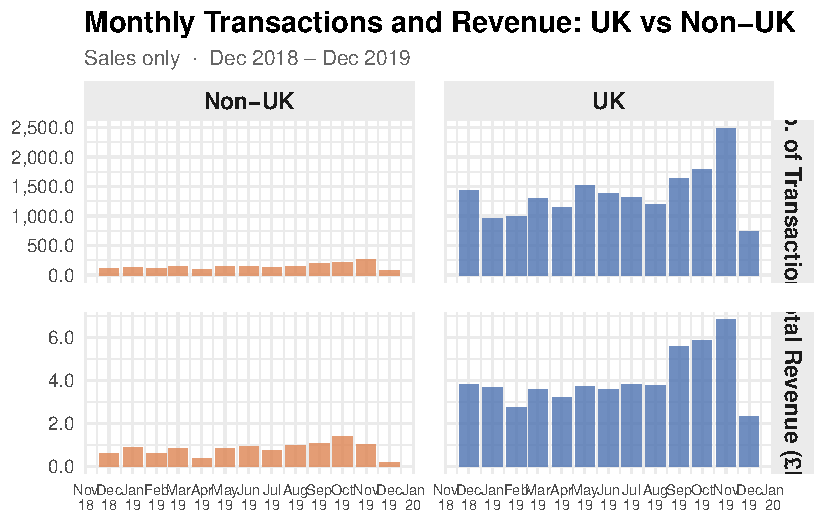
\includegraphics[keepaspectratio]{report_files/figure-pdf/fig-overview-1.pdf}}

}

\caption{\label{fig-overview}Monthly Transaction and Revenue in UK vs
non-UK countries in 2018-2019 period}

\end{figure}%

\subsection{Results}\label{results}

\subsubsection{Number of orders and total Volume by
month}\label{number-of-orders-and-total-volume-by-month}

As presented in Figure~\ref{fig-overview}, The UK market consistently
dominated in both number of transactions and revenue throughout the
recorded period. A pronounced upward trend is observed from September
2019 onwards, with transactions and revenue in the UK peaking in
November 2019 at nearly 2500 orders and approximately £6.8M
respectively, likely driven by seasonal demand ahead of the holiday
period.

The Non-UK market, while significantly smaller in absolute scale,
demonstrated a gradual growth trajectory across 2019 with the upward
trend merely mirror UK market. This suggests a slow but steady expansion
of the international customer base.

Figure~\ref{fig-non-uk-figures} shows the top non-UK countries by
revenue amount, and also hints at an interesting idea; that the retailer
is performing very well in some countries despite relatively low numbers
of transactions. This will be covered in more depth in
Section~\ref{sec-basket-values}.

\begin{figure}

\centering{

\pandocbounded{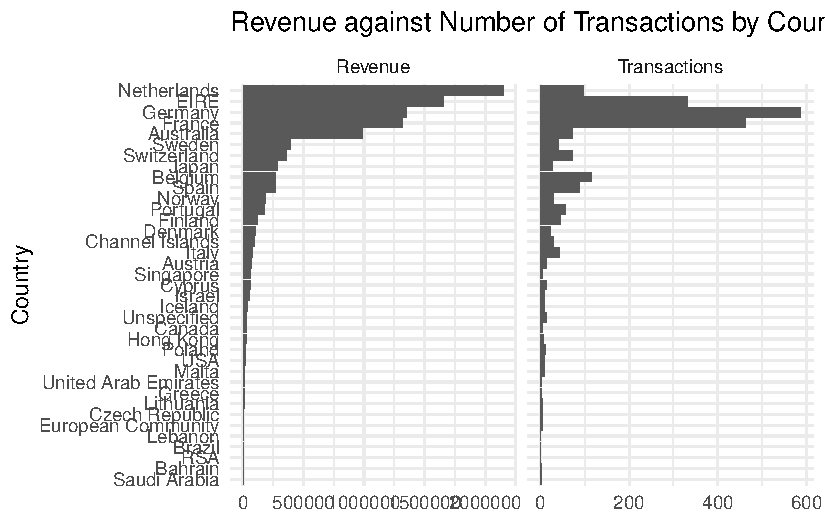
\includegraphics[keepaspectratio]{report_files/figure-pdf/fig-non-uk-figures-1.pdf}}

}

\caption{\label{fig-non-uk-figures}Transactions and Revenue for Non-UK
Countries}

\end{figure}%

\subsubsection{General Quantitative
metrics}\label{general-quantitative-metrics}

As seen in Figure~\ref{fig-overview}, both the UK and Non-UK markets
reached their peak transaction volumes and revenue towards the end of
2019. Referencing Table~\ref{tbl-overview}, the UK reached 2487
transactions and £6.81M in revenue in November 2019, while Non-UK
countries peaked at 266 transactions in the same month. This Q4 surge is
consistent with seasonal holidays like Christmas and New Year.

Notably, Non-UK maximum revenue occurred in October 2019 (£1.37M) rather
than November despite November having more transactions, suggesting a
higher average basket value per order in October.

The minimum values for both regions fall in December 2019 across all
metrics. This might not be a genuine business downturn but rather a data
artefact, as December 2019 represents an incomplete month in the
dataset.

\begingroup\fontsize{13}{15}\selectfont

\begin{longtable}[t]{>{}lrr}

\caption{\label{tbl-overview}Monthly Transaction and Revenue in UK vs
non-UK countries in 2018-2019 period}

\tabularnewline

\toprule
\multicolumn{1}{c}{ } & \multicolumn{2}{c}{Region} \\
\cmidrule(l{3pt}r{3pt}){2-3}
\cellcolor[HTML]{4C72B0}{\textcolor{white}{\textbf{Metric}}} & \cellcolor[HTML]{4C72B0}{\textcolor{white}{\textbf{Non-UK}}} & \cellcolor[HTML]{4C72B0}{\textcolor{white}{\textbf{UK}}}\\
\midrule
\textbf{Total Transactions} & 1,882 & 17,908\\
\textbf{Mean Transactions/Month} & 145 & 1,378\\
\textbf{Min Transactions/Month} & 73 & 744\\
\textbf{Max Transactions/Month} & 266 & 2,487\\
\textbf{Total Revenue (£)} & 10,434,508.94 & 52,346,877.60\\
\addlinespace
\textbf{Mean Revenue/Month (£)} & 802,654.53 & 4,026,682.89\\
\textbf{Min Revenue/Month (£)} & 182,853.09 & 2,329,216.43\\
\textbf{Max Revenue/Month (£)} & 1,374,514.18 & 6,806,782.19\\
\bottomrule

\end{longtable}

\endgroup{}

\subsubsection{Countries' basket value}\label{sec-basket-values}

Figure~\ref{fig-basket-value} presents basket size statistics across top
10 countries with the biggest basket and the UK. Netherlands, Australia
and Singapore recorded the highest mean basket values at £22888, £16055
and £15870 respectively. Notably, these countries achieved these values
from a very small number of transactions, especially Singapore had only
4 transactions, this pattern could indicate wholesale or B2B purchasing
behaviour rather than individual retail orders.

\begin{figure}

\centering{

\pandocbounded{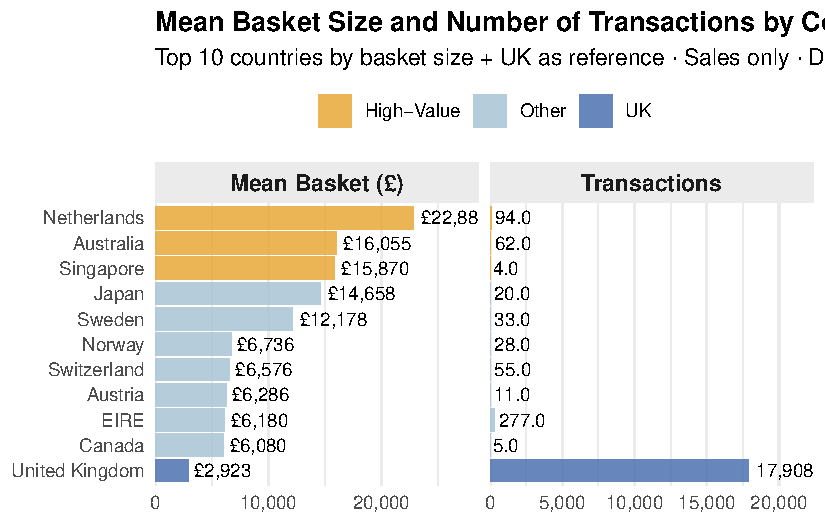
\includegraphics[keepaspectratio]{report_files/figure-pdf/fig-basket-value-1.pdf}}

}

\caption{\label{fig-basket-value}Metrics for Basket Size per transaction
by country in 2018-2019 period}

\end{figure}%

\subsubsection{Cancelled orders insight}\label{cancelled-orders-insight}

Figure~\ref{fig-cancellation} shows that the USA has the highest
cancellation rate at 29.63\%, followed by Malta (9.4\%) and Japan
(9.16\%), all well above the UK benchmark of 1.52\%. However, despite
its low rate, the UK incurs the largest revenue loss at £2509.3K due to
its transaction number. Among Non-UK markets, EIRE (Ireland) records the
highest revenue lost at £52.8K, making it the most financially impactful
cancellation market outside the UK.

\begin{figure}

\centering{

\pandocbounded{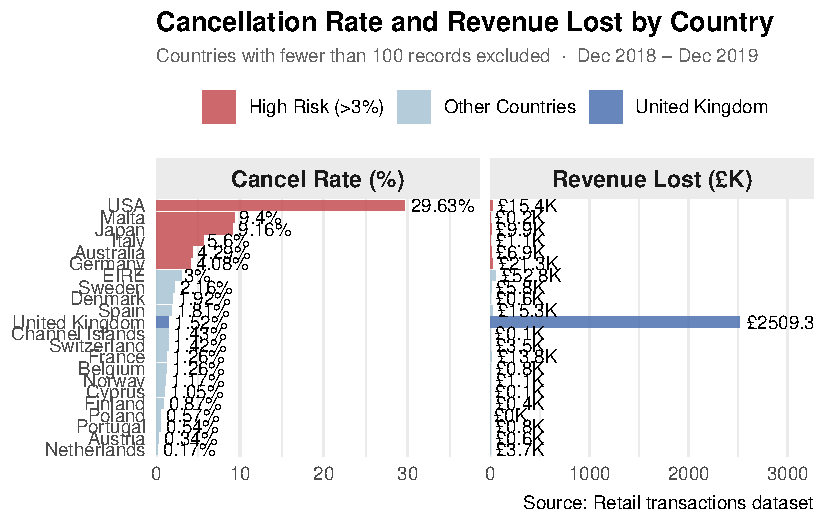
\includegraphics[keepaspectratio]{report_files/figure-pdf/fig-cancellation-1.pdf}}

}

\caption{\label{fig-cancellation}Cancellation rate and Revenue lost by
each Country}

\end{figure}%

\subsection{Dicussion}\label{dicussion}

The results indicates that this business is operationally strong in its
domestic market but has significant untapped potential internationally.

\subsubsection{General market is
Seasonal}\label{general-market-is-seasonal}

The dominant Q4 seasonality observed in Figure~\ref{fig-overview}
suggests the business is \textbf{heavily reliant on the festive season
period} to drive annual performance. While this concentration generates
strong peak revenue, it also \textbf{exposes the business to seasonal
risk}.

\subsubsection{High value international B2B
market}\label{high-value-international-b2b-market}

The basket size analysis in Figure~\ref{fig-basket-value} reveals a more
complex international picture. Despite lower transaction volumes, most
\textbf{Non-UK customers spend nearly exponentially more per order
comparing to the UK}. Countries such as the Netherlands, Singapore, and
Australia demonstrate average basket sizes of approximately £16000,
mostly indicate that they belong to the \textbf{B2B customer segment}.
Rather than casual retail consumers, these clients are bulk purchasers
placing infrequent, high-value orders, making them disproportionately
valuable relative to their transaction volume.

\subsubsection{Barrier regarding international
sales}\label{barrier-regarding-international-sales}

However, Figure~\ref{fig-cancellation} highlights a key operational
challenge in international markets. The cancellation rate at the USA
(29.6\%), Japan (9.2\%) and Germany (4.1\%) all exceed the UK benchmark
of 1.52\%, suggesting that international fulfilment reliability remains
inconsistent. While EIRE represents the largest Non-UK revenue loss at
£52.8K, the high-rate markets like the USA likely reflect \textbf{demand
uncertainty} or \textbf{logistics hindrance} rather than product
dissatisfaction.

\subsection{Recommendation}\label{recommendation}

\textbf{Reduce seasonal dependency:} The business should invest in
mid-year promotional campaigns, particularly in months of February and
April while they showed the modest number, to reduce the financial risk
of a single underperforming holiday season.

\textbf{Formalise and grow the international wholesale channel:} The
high basket sizes recorded in the Netherlands, Australia and Singapore
signal an existing wholesale customer base. Rather than treating these
as ordinary transactions, the business should \emph{develop a dedicated
B2B programme with volume-based pricing, account management and tailored
outreach}.

\textbf{Address international fulfilment gaps before scaling:} The
elevated cancellation rates in some countries suggest that the
operational infrastructure for international orders is not yet mature.
Before investing further in these markets, the business should
investigate the \emph{root causes of cancellations: whether driven by
shipping delays, product mismatches, or payment friction}. The
Netherlands, with a near-zero cancellation rate of 0.17\%, offers a
useful operational benchmark for what reliable international fulfilment
looks like.

\subsection{References}\label{references}

\protect\phantomsection\label{refs}
\begin{CSLReferences}{1}{0}
\bibitem[\citeproctext]{ref-janitor-cite}
Firke, S. (2024). \emph{Janitor: Simple tools for examining and cleaning
dirty data}. \url{https://doi.org/10.32614/CRAN.package.janitor}

\bibitem[\citeproctext]{ref-lubridate-cite}
Grolemund, G., \& Wickham, H. (2011). Dates and times made easy with
{lubridate}. \emph{Journal of Statistical Software}, \emph{40}(3),
1--25. \url{https://www.jstatsoft.org/v40/i03/}

\bibitem[\citeproctext]{ref-ramos_e-commerce_nodate}
Ramos, G. (n.d.). \emph{E-commerce {Business} {Transaction}}. Retrieved
June 6, 2026, from
\url{https://www.kaggle.com/datasets/gabrielramos87/an-online-shop-business}

\bibitem[\citeproctext]{ref-renv-cite}
Ushey, K., \& Wickham, H. (2026). \emph{Renv: Project environments}.
\url{https://doi.org/10.32614/CRAN.package.renv}

\bibitem[\citeproctext]{ref-tidyverse-cite}
Wickham, H., Averick, M., Bryan, J., Chang, W., McGowan, L. D.,
François, R., Grolemund, G., Hayes, A., Henry, L., Hester, J., Kuhn, M.,
Pedersen, T. L., Miller, E., Bache, S. M., Müller, K., Ooms, J.,
Robinson, D., Seidel, D. P., Spinu, V., \ldots{} Yutani, H. (2019).
Welcome to the {tidyverse}. \emph{Journal of Open Source Software},
\emph{4}(43), 1686. \url{https://doi.org/10.21105/joss.01686}

\bibitem[\citeproctext]{ref-scales-cite}
Wickham, H., Pedersen, T. L., \& Seidel, D. (2025). \emph{Scales: Scale
functions for visualization}.
\url{https://doi.org/10.32614/CRAN.package.scales}

\bibitem[\citeproctext]{ref-knitr-cite}
Xie, Y. (2025). \emph{Knitr: A general-purpose package for dynamic
report generation in {R}}. \url{https://yihui.org/knitr/}

\bibitem[\citeproctext]{ref-kableExtra-cite}
Zhu, H. (2024). \emph{kableExtra: Construct complex table with 'kable'
and pipe syntax}. \url{https://doi.org/10.32614/CRAN.package.kableExtra}

\end{CSLReferences}




\end{document}
